\documentclass{article} 
\usepackage[left=0.75in,top=0.6in,right=0.75in,bottom=0.6in]{geometry} % Document margins
\usepackage{tabularx}
\usepackage{fancyvrb}
%\usepackage[hidelinks]{hyperref}
\usepackage{graphicx}
\usepackage{float}
\usepackage{fancyhdr}
\usepackage{geometry}
\usepackage{lastpage}
\usepackage{tabu}
\usepackage{hyperref}



\geometry{
  top=1in,            % <-- you want to adjust this
  inner=0.5in,
  outer=0.5in,
  bottom=1in,
  headheight=5ex,       % <-- and this
  headsep=4ex,          % <-- and this
}

\pagestyle{fancy}
\fancyhf{}
\rhead{\Large\textit{Old Dominion University}}
\lhead{\Large\textit{ECE 432: Assignment 9}}
\cfoot{Page \thepage \hspace{1pt} of \pageref{LastPage}}
\renewcommand{\footrulewidth}{1pt}

\begin{document}

%----------------------------------------------------------------------------------------
%		 TITLE PAGE
%----------------------------------------------------------------------------------------

\begin{titlepage}

\vspace*{45 pt}
\begin{center}
\Huge{\bf CS 432/532:  Web Science}\\
\huge{Spring 2017\\}

\vspace{60 pt}
\Huge\underline {Assignment 9}\\

\vspace{10 pt}
\Huge{Michael Micros}\\\

{\Large \bf {Instructor: Michael L. Nelson}}\\

\vspace{230 pt}
{\huge \bf {Old Dominon University}}\\
{\huge \bf {Norfolk, Virginia}}\\

\vspace{10 pt}
\today

\end{center}
\end{titlepage}




%----------------------------------------------------------------------------------------
%		PROBLEM 1
%----------------------------------------------------------------------------------------

\section*{{\underline{\huge {Problem 1:}} Choosing a blog and classifying entries}}

I originally ``claimed" the headlines newsfeed from foxsports.com. Apparently, foxsports uses rss and not atom, which created a lot of difficulties for me. After battling with pagination for a while I decided to switch to a sports blog that I discovered, which coincidentally is very interesting and I believe ties in with this class to a certain degree. This blog is :

 http://thehothand.blogspot.com/ \\
This blog is writen by Texas Tech Professor Alan Reifman and its topic is statistical analysis of streaks in sports.
In order to get the xml for 100 entries from the blog the following cURL command was used:

\begin{figure} [H]
 \centering
 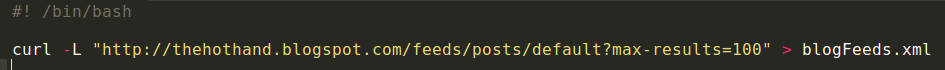
\includegraphics[width=\linewidth]{getblog.png}
 % \caption{Layout of the GUI produced by the Qt program}
\end{figure}

``blogFeeds.txt" was uploded to github. Additionally, the classification of the entries of the feed are in ``classifications.txt".

\begin{figure} [H]
 \centering
 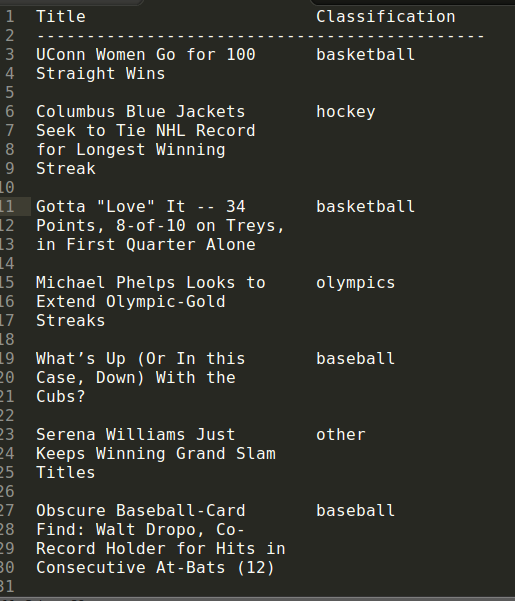
\includegraphics[height = 10 cm]{classifications.png}
 \caption{Sample of classifyed entries from the ``hothand" blog. }
\end{figure}

The categories that I created were:

\begin{itemize}
  \item   basketball
  \item   baseball
  \item   hockey
  \item   olympics
  \item   other
\end{itemize}

It is important to note that about 80\% of this blog deals with streaks in basketbal and baseball. Therefore, I had to put tennis, footbal( suprizingly) and soccer in the ``others" category, so as to limit the number of categories but also because there were so few entries in these categories.
%----------------------------------------------------------------------------------------
%		PROBLEM 2
%----------------------------------------------------------------------------------------

\section*{{\underline{\huge {Problem 2:}} Training and Testing (50-50)  }}
Making use of the code provided by the ``Programming Collective Intelligence" textbook we train the Fisher classifier on the first 50 entries and test it on the final 50. The feedfilter and docclass modules were imported to perform this. The code for this question and question 3 is ``part1.py". The only parameter changed is the number of entries to use for training.The classifications for all the entries were saved in ``class.txt" and loaded to the script.

\begin{figure} [H]
 \centering
 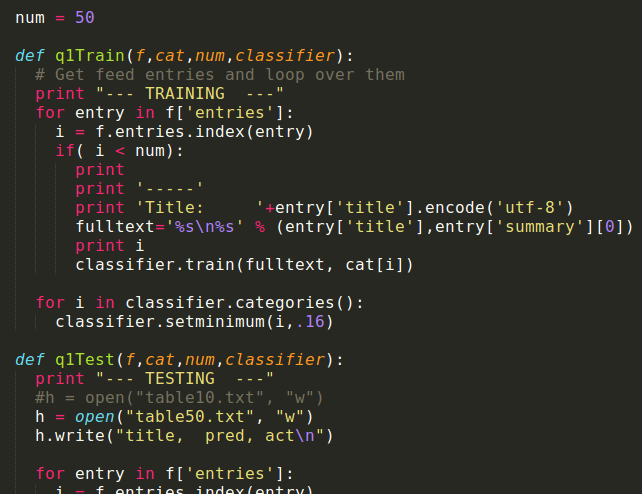
\includegraphics[height = 10 cm]{p1.png}
 \caption{Part of ``part1.py" code that trains and tested the Fisher classifyer.}
\end{figure}

The precision, and f-measure were calculated using the ``assess" function displayed in Fig 4.\\

Precision: 0.88

Recal: 0.96

F-Measure: 0.92\\
The classification results were saved in ``table50.txt" and uploaded to github.
\begin{figure} [H]
 \centering
 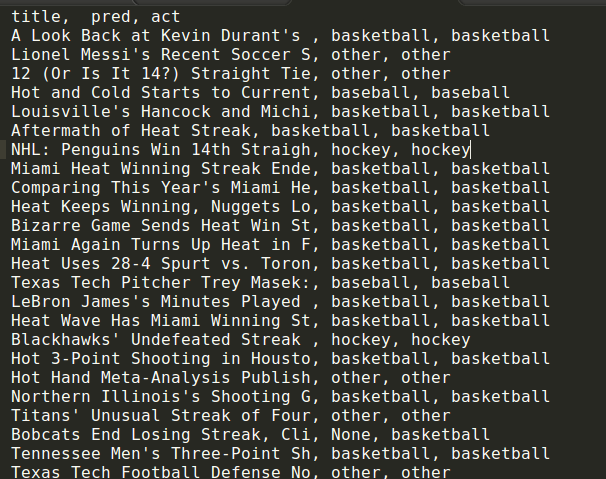
\includegraphics[height = 10 cm]{res1.png}
 \caption{Part of the results of the 50 entries the classifier was tested on.}
\end{figure}


\begin{figure} [H]
 \centering
 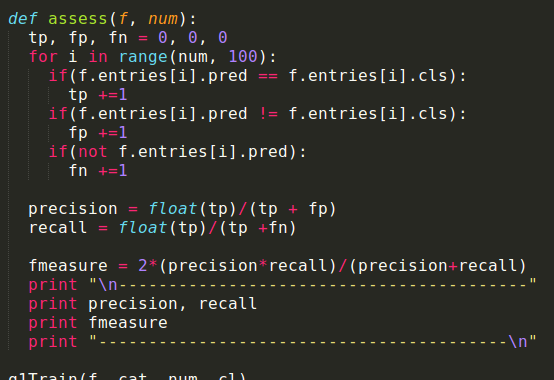
\includegraphics[height = 10 cm]{assfun.png}
 \caption{The assess function that calculates precision, recall and f-measure}
\end{figure}


%----------------------------------------------------------------------------------------
%		PROBLEM 3
%----------------------------------------------------------------------------------------

\section*{{\underline{\huge {Problem 3:}} Training and Testing (90-10) }}
The same script used earlier is modifyed to train on the first 90 entries and test on the final 10.\\
The results calculated for a 90-10 split were saved in ``table10.txt".

Precision: 0.6

Recal: 0.86

F-Measure: 0.71\\

The fact that the 90-10 split performs worse than the 50-50, I beleive has to do with the nature of the entries. Most of the data fall under the category of basketball and baseball. Additionally, most of the entries that belong in the ``olympics" category are in the last 10 entries that we test. I feel that we have fallen into one of those exceptions where the training set does not apply nicely to the testing data. A 10-fold cross-validation would probably provide more realistic results.

\begin{figure} [H]
 \centering
 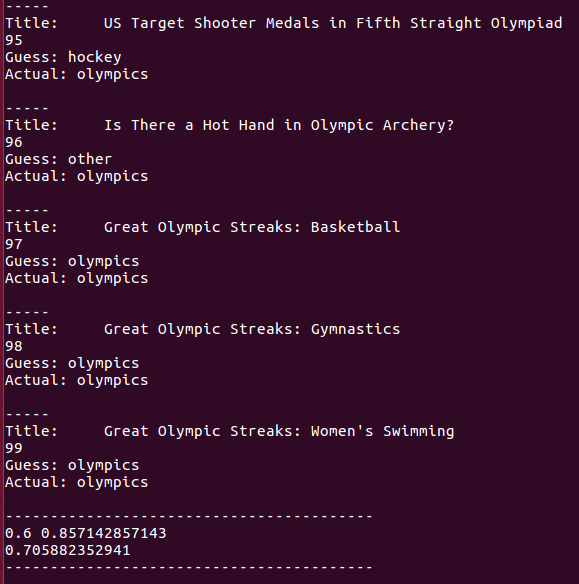
\includegraphics[height = 10 cm]{res2.png}
 \caption{table10.txt}
\end{figure}

\begin{figure} [H]
 \centering
 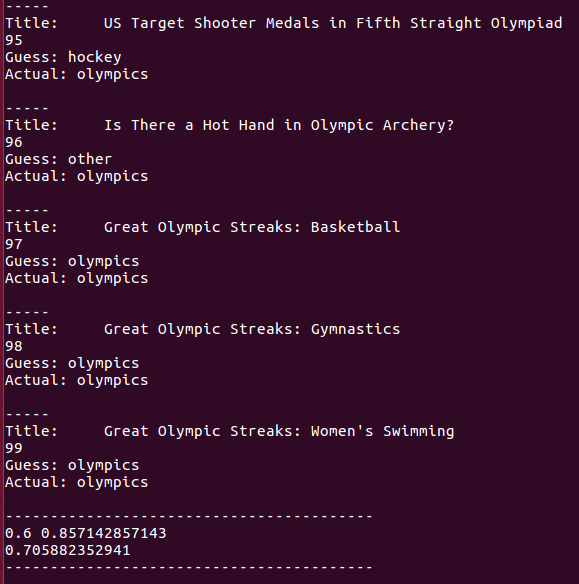
\includegraphics[height = 10 cm]{res2.png}
 \caption{table10.txt}
\end{figure}






%----------------------------------------------------------------------------------------
\end{document}
